Lo scopo di questa esperienza è la valutazione dello \textbf{slew-rate} dell’amplificatore operazionale LM741CN, mediante l’utilizzo di un circuito buffer inseguitore (di tensione).\\ Il circuito, riportato in Figura \ref{fig:Circuito3}, è alimentato dalla tensione duale $\pm V_{CC}=\pm 10V$.
\begin{figure}[h]
    \centering
    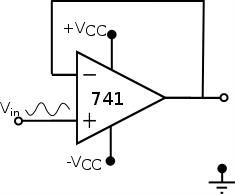
\includegraphics{images/Circuit3.png}
    \caption{Schema circuito}
    \label{fig:Circuito3}
\end{figure}
\subsection{Assemblaggi e settaggi}
Si riporta in Figura \ref{fig:LabCircuit3} il setup sperimentale, con ingresso $V_{in}$ connesso - mediante "T" - al generatore di forma d'onda e uscita $V_{out}$ connessa la canale 2 dell'oscilloscopio.
\begin{figure}[H]
    \centering
    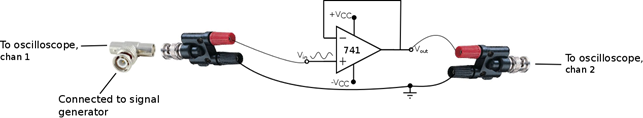
\includegraphics[width=0.8\linewidth]{images/LabCircuit3.png}
    \caption{Schema di collegamento}
    \label{fig:LabCircuit3}
\end{figure}
Il generatore di forme d'onda è stato impostato per fornire in uscita la forma d'onda con le seguenti caratteristiche:
\begin{itemize}
    \item Forma d'onda: quadra
    \item Frequenza: 20 kHz
    \item Tensione picco-picco: $10V$
    \item Duty-cycle: 50\%
\end{itemize}
\subsection{Procedura di valutazione e risultati}
Tramite i cursori dell' oscilloscopio è stato misurato lo slew rate, come si vede in Figura \ref{fig:Ris3}
\begin{figure}[H]
    \centering
    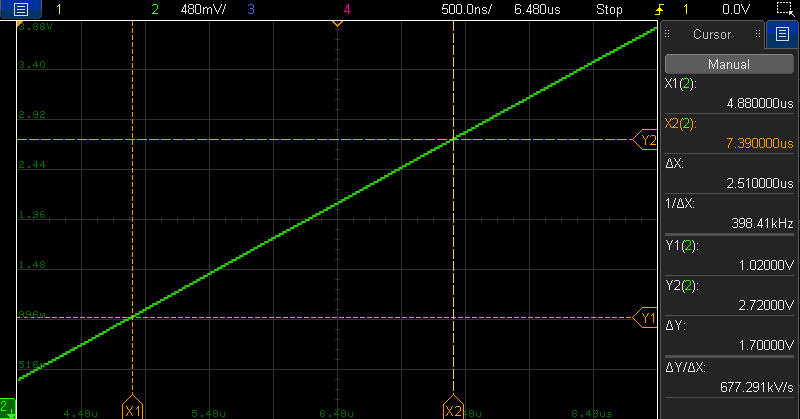
\includegraphics[width=\linewidth]{images/Ris3.png}
    \caption{Misura dello slew rate dall'oscilloscopio}
    \label{fig:Ris3}
\end{figure}
Il cui valore è
\begin{equation}
    \text{SlewRate} = 0.6773V/\mu s
\end{equation}